\begin{name}
	{ÔN TẬP KIỂM TRA CUỐI HỌC KÌ 1 - KNTT}
	{TOÁN 10}
	{LỚP TOÁN THẦY PHÁT}
	{\thoigian}
\end{name}

%================================PHẦN I
\caulc
\Opensolutionfile{ans}[ans/0-HK1-KN-5-SocSon-HaNoi-2324-Phan-I]
\setcounter{ex}{0}

%==========Câu 1
\begin{ex}%[0-HK1-KN-5-SocSon-HaNoi-2324]%[VN-MT-6,VM024]%[0D6H1-4]
	Chiều dài của một cây cầu là $\ell=1\,547{,}25\mathrm{~m}\pm 0{,}01\mathrm{~m}$. Hãy cho biết số quy tròn của $\ell$.
	\choice
	{$1\,548$ m}
	{$1\,547$ m}
	{\True $1\,547{,}3$ m}
	{$1\,547{,}2$ m}
	\loigiai{
		Vì $\ell=1\,547{,}25\mathrm{~m}\pm 0{,}01\mathrm{~m}$ nên ta quy tròn $\ell$ đến chữ số thập phân thứ nhất.\\
		Vậy $\ell\approx 1\,547{,}3$ m.
	}
\end{ex}
%==========Câu 2
\begin{ex}%[0-HK1-KN-5-SocSon-HaNoi-2324]%[VN-MT-6,VM024]%[0H5N1-1]
	Cho hai điểm phân biệt $A$ và $B$, số vectơ khác vectơ-không có thể xác định được từ hai điểm $A$ và $B$ là
	\choice
	{$4$}
	{$3$}
	{\True $2$}
	{$1$}
	\loigiai{
		Từ hai điểm phân biệt $A$ và $B$ ta xác định được hai vectơ là $\overrightarrow{AB}$ và $\overrightarrow{BA}$.
	}
\end{ex}
%==========Câu 3
\begin{ex}%[0-HK1-KN-5-SocSon-HaNoi-2324]%[VN-MT-6,VM024]%[0H9H1-3]
	Trong mặt phẳng với hệ tọa độ $Oxy$, cho ba điểm $A(1;1)$, $B(3;2)$, $C(6;5)$. Tìm tọa độ điểm $D$ để $ABCD$ là hình bình hành.
	\choice
	{\True $(4;4)$}
	{$(3;4)$}
	{$(4;3)$}
	{$(8;6)$}
	\loigiai{
		Ta có $\overrightarrow{AB}=(2;1)$, $\overrightarrow{BC}=(3;3)$. Ta thấy $\dfrac{2}{3}\ne\dfrac{1}{3}$ nên hai vectơ $\overrightarrow{AB}$ và $\overrightarrow{BC}$ không cùng phương. Do đó, ba điểm $A$, $B$, $C$ không thẳng hàng.\\
		Gọi $D(x;y)$. Khi đó, $\overrightarrow{AD}=(x-1;y-1)$.\\
		$ABCD$ là hình bình hành khi và chỉ khi $\overrightarrow{AD}=\overrightarrow{BC}$ $\Leftrightarrow$ $\heva{&x-1=3\\ &y-1=3}$ $\Leftrightarrow$ $\heva{&x=4\\ &y=4.}$\\
		Vậy $D(4;4)$.
	}
\end{ex}
%==========Câu 4
\begin{ex}%[0-HK1-KN-5-SocSon-HaNoi-2324]%[VN-MT-6,VM024]%[0D1N1-3]
	Cho mệnh đề $A\colon$ \lq\lq$\forall x\in\mathbb{R}$, $x^2-x+7<0$\rq\rq. Mệnh đề phủ định của $A$ là mệnh đề
	\choice
	{$\forall x\in\mathbb{R}$, $x^2-x+7>0$}
	{\True $\exists x\in\mathbb{R}$, $x^2-x+7\ge 0$}
	{$\exists x\in\mathbb{R}$, $x^2-x+7>0$}
	{$\forall x\in\mathbb{R}$, $x^2-x+7\le 0$}
	\loigiai{
		Mệnh đề phủ định của mệnh đề \lq\lq$\forall x\in\mathbb{R}$, $x^2-x+7<0$\rq\rq~là mệnh đề \lq\lq$\exists x\in\mathbb{R}$, $x^2-x+7\ge 0$\rq\rq.
	}
\end{ex}
%==========Câu 5
\begin{ex}%[0-HK1-KN-5-SocSon-HaNoi-2324]%[VN-MT-6,VM024]%[0D2N1-1]
	Bất phương trình nào say đây là bất phương trình bậc nhất hai ẩn $x$, $y$?
	\choice
	{$64 x^2+y>8$}
	{$xy+4y<-3$}
	{\True $2x-3y\ge 5$}
	{$2x-5 y^2\ge 6$}
	\loigiai{
		Bất phương trình bậc nhất hai ẩn $x$, $y$ có dạng tổng quát là $ax+by\le0$ (hoặc $ax+by\ge0$, hoặc $ax+by <0$, hoặc $ax+by >0$), trong đó $a$, $b$, $c$ là những số thực đã cho, $a$ và $b$ không đồng thời bằng $0$ nên chỉ có duy nhất một bất phương trình $2x-3y\ge 5$ là bất phương trình bậc nhất hai ẩn $x$, $y$.
	}
\end{ex}
%==========Câu 6
\begin{ex}%[0-HK1-KN-5-SocSon-HaNoi-2324]%[VN-MT-6,VM024]%[0D6N3-3]
	Điểm kiểm tra môn Toán của một nhóm gồm $10$ học sinh được ghi lại trong bảng sau
	\begin{center}
		\begin{tabular}{|c|c|c|c|c|c|c|c|c|c|}
			\hline
			$3$ & $4$ & $4{,}5$ & $5$ & $6$ & $6{,}5$ & $8$ & $8{,}5$ & $9$ & $10$ \\ \hline
		\end{tabular}
	\end{center}
	Tìm trung vị của mẫu số liệu trên.
	\choice
	{$6$}
	{$6{,}5$}
	{$8$}
	{\True $6{,}25$}
	\loigiai{
		Mẫu số liệu đã cho đã được sắp xếp theo thứ tự không giảm và số các giá trị của mẫu số liệu là $10$ nên có trung vị là $\mathrm{M}_{\mathrm{e}}=\dfrac{x_5+x_6}{2}=\dfrac{6+6{,}5}{2}=6{,}25$.
	}
\end{ex}
%==========Câu 7
\begin{ex}%[0-HK1-KN-5-SocSon-HaNoi-2324]%[VN-MT-6,VM024]%[0D1N2-2]
	Trong các tập sau, tập hợp nào có đúng một tập hợp con?
	\choice
	{$\left\{\varnothing\right\}$}
	{$\left\{a;\varnothing\right\}$}
	{\True $\varnothing$}
	{$\left\{a\right\}$}
	\loigiai{
		Ta biết rằng tập hợp rỗng là tập hợp con của mọi tập hợp và mỗi tập hợp $A$ đều là tập con của chính nó. Do đó, tập hợp có đúng một tập hợp con khi và chỉ khi nó là tập rỗng $\varnothing$.\\
		Chú ý rằng tập hợp $\left\{\varnothing\right\}$ là một hợp gồm một phần tử mà phần tử đó là một tập hợp (tập $\varnothing$), tập hợp này khác với tập rỗng.
	}
\end{ex}
%==========Câu 8
\begin{ex}%[0-HK1-KN-5-SocSon-HaNoi-2324]%[VN-MT-6,VM024]%[0D2H2-2]
	\immini[thm]{Miền trong của tam giác $OAB$ (kể cả ba cạnh) trong hình bên là miền nghiệm của hệ bất phương trình nào trong bốn phương án dưới đây?
		\choice
		{\True $\heva{& x\ge 0\\ & y\ge 0\\ & x+y\le 2}$}
		{$\heva{& x\ge 0\\ & y\ge 0\\ & x+y\le -2}$}
		{$\heva{& x\ge 0\\ & y\ge 0\\ & x+y\ge -2}$}
		{$\heva{& x\ge 0\\ & y\ge 0\\ & x+y\ge 2}$}}
	{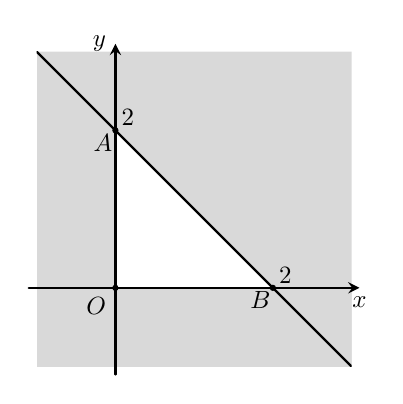
\begin{tikzpicture}[line join=round, line cap=round,>=stealth,thick]
			\tikzset{every node/.style={scale=0.9}}
			\begin{scope}
				\clip (-1,-1) rectangle (3,3);
				\fill[gray!30] (-1,-1) rectangle (0,3);
				\fill[gray!30] (-1,3)--(3,-1)--(3,3)--cycle;
				\fill[gray!30] (-1,-1) rectangle (3,0);
				\draw (-1,3)--(3,-1);
			\end{scope}
			\draw[->] (-1.1,0)--(3.1,0) node[below]{$x$};
			\draw[->] (0,-1.1)--(0,3.1) node[left]{$y$};
			\fill (0,0)circle(0.04) node[below left]{$O$};
			\fill (0,2)circle(0.04)node[shift={(-135:.25)}]{$A$};
			\fill (2,0)circle(0.04)node[shift={(-135:.25)}]{$B$};
			\path(0,2)node[shift={(45:.25)}]{$2$};
			\path(2,0)node[shift={(45:.25)}]{$2$};
	\end{tikzpicture}}
	\loigiai{
		Miền nghiệm của hệ nằm bên phải trục tung nên $x\ge0$;\\
		Miền nghiệm của hệ nằm phía trên trục hoành nên $y\ge0$;\\
		Đường thẳng $AB$ đi qua điểm $A(0;2)$ nên loại hai hệ $\heva{& x\ge 0\\ & y\ge 0\\ & x+y\le -2}$ và $\heva{& x\ge 0\\ & y\ge 0\\& x+y\ge -2.}$\\
		Vì điểm $M\left(\dfrac{1}{2};\dfrac{1}{2}\right)$ nên chọn $\heva{& x\ge 0\\ & y\ge 0\\ & x+y\le 2.}$
	}
\end{ex}
%==========Câu 9
\begin{ex}%[0-HK1-KN-5-SocSon-HaNoi-2324]%[VN-MT-6,VM024]%[0D2H2-2]
	Cặp số nào sau đây \textbf{không phải} là nghiệm của hệ bất phương trình $\heva{& x+y\ge 1\\ & 2x-y\le 4}$?
	\choice
	{$(3;2)$}
	{\True $(0;-2)$}
	{$(0;5)$}
	{$(2;4)$}
	\loigiai{
		Lần lượt thay các cặp số $(3;2)$, $(0;-2)$, $(0;5)$, $(2;4)$ vào hệ bất phương trình $\heva{& x+y\ge 1\\ & 2x-y\le 4}$, ta thấy chỉ có cặp số $(0;-2)$ không thỏa mãn hệ.
	}
\end{ex}
%==========Câu 10
\begin{ex}%[0-HK1-KN-5-SocSon-HaNoi-2324]%[VN-MT-6,VM024]%[0D6N4-1]
	Số đặc trưng nào sau đây đo độ phân tán của mẫu số liệu?
	\choice
	{\True Độ lệch chuẩn}
	{Mốt}
	{Trung vị}
	{Số trung bình}
	\loigiai{
		Khoảng biến thiên, khoảng tứ phân vị, phương sai và độ lệch chuẩn là các số đặc trưng đo độ phân tán của mẫu số liệu.
	}
\end{ex}
%==========Câu 11
\begin{ex}%[0-HK1-KN-5-SocSon-HaNoi-2324]%[VN-MT-6,VM024]%[0D2H2-3]
	Bác An dự định để $x$ sào đất trồng cà tím và $y$ sào đất trồng cà chua. Bác dự định để tối đa $10$ triệu đồng để mua hạt giống. Tiền mua hạt giống cà tím là $200\, 000$ đồng/sào và cà chua là $100\, 000$ đồng/sào. Hệ phương trình mô tả điều kiện của $x$, $y$ là
	\choice
	{$\heva{& 2x+y\ge 100\\ & x\ge 0\\ & y\ge 0}$}
	{$\heva{& x+2y\le 100\\ & x\ge 0\\ & y\ge 0}$}
	{\True $\heva{& 2x+y\le 100\\ & x\ge 0\\ & y\ge 0}$}
	{$\heva{& 2x+y\le 1\, 000\\ & x\ge 0\\ & y\ge 0}$}
	\loigiai{
		Diện tích đất trồng cà tím và cà chua là các số không âm nên $x\ge0$, $y\ge0$.\\
		Vì tiền mua hạt giống cà tím là $200\, 000$ đồng/sào, cà chua là $100\, 000$ đồng/sào và số tiền tối đa là $10$ triệu đồng nên $200\, 000x+100\, 000y\le 10\, 000\, 000$ $\Leftrightarrow$ $2x+y\le100$.\\
		Vậy hệ phương trình mô tả điều kiện của $x$, $y$ là $\heva{& 2x+y\le 100\\ & x\ge 0\\ & y\ge 0.}$
	}
\end{ex}
%==========Câu 12
\begin{ex}%[0-HK1-KN-5-SocSon-HaNoi-2324]%[VN-MT-6,VM024]%[0H4N1-3]
	Hai góc nhọn $\alpha$ và $\beta$ phụ nhau, hệ thức nào sau đây là \textbf{sai}?
	\choice
	{$\tan\alpha =\cot\beta$}
	{$\cot\alpha =\dfrac{1}{\cot\beta}$}
	{$\sin\alpha =\cos\beta$}
	{\True $\cos\alpha =-\sin\beta$}
	\loigiai{
		Vì $\alpha$ và $\beta$ là hai góc nhọn phụ nhau nên $\alpha=90^\circ-\beta$. Do đó,
		\allowdisplaybreaks
		\begin{eqnarray*}
			&&\tan\alpha=\tan(90^\circ-\beta)=\cot\beta;\\
			&&\cot\alpha=\cot(90^\circ-\beta)=\tan\beta=\dfrac{1}{\cot\beta};\\
			&&\sin\alpha=\sin(90^\circ-\beta)=\cos\beta;\\
			&&\cos\alpha=\cos(90^\circ-\beta)=\sin\beta\ne-\sin\beta.
		\end{eqnarray*}
	}
\end{ex}
\Closesolutionfile{ans}
%================================PHẦN II
\cauds
\Opensolutionfile{ans}[ans/0-HK1-KN-5-SocSon-HaNoi-2324-Phan-II]
\setcounter{ex}{0}

%==========Câu 1
\begin{ex}%[0-HK1-KN-5-SocSon-HaNoi-2324]%[VN-MT-6,VM024]%[0D6H4-4]
	Sải cánh (tính theo đơn vị cm) của $90$ con chim sẻ được thống kê và ghi lại trong bảng dưới đây
	\begin{center}
		\begin{tabular}{|l|c|c|c|c|c|c|c|c|c|c|}
			\hline
			Sải cánh & $18$ & $19$ & $20$ & $21$ & $22$ & $23$ & $24$\\ \hline
			Số lượng & $6$ & $11$ & $19$ & $20$ & $15$ & $12$ & $7$\\ \hline
		\end{tabular}
	\end{center}
	\choiceTF
	{Mốt của mẫu số liệu là $20$}
	{\True Khoảng biến thiên của mẫu số liệu là $6$}
	{\True Số trung bình của mẫu số liệu gần bằng $21{,}01$}
	{Độ lệch chuẩn của mẫu số liệu gần bằng $2{,}73$}
	\loigiai{
		\begin{itemchoice}
			\itemch \textbf{Sai}.\\
			Mốt của một mẫu số liệu là giá trị có tần số lớn nhất. Do đó, mốt của mẫu số liệu này là $21$.
			\itemch \textbf{Đúng}.\\
			Khoảng biến thiên của mẫu số liệu là $R=24-18=6$.
			\itemch \textbf{Đúng}.\\
			Số trung bình là $\overline{x}=\dfrac{1}{90}(6\cdot18+11\cdot19+19\cdot20+20\cdot21+15\cdot22+12\cdot23+7\cdot24)\approx 21{,}01$.
			\itemch \textbf{Sai}.\\
			Phương sai là
			\allowdisplaybreaks
			\begin{eqnarray*}
				s^2&=&\dfrac{6(18-21{,}01)^2+11(19-21{,}01)^2+19(20-21{,}01)^2+20(21-21{,}01)^2}{90}+\\
				&&+\dfrac{15(22-21{,}01)^2+12(23-21{,}01)^2+7(24-21{,}01)^2}{90}\\
				&\approx& 2{,}6999.
			\end{eqnarray*}
			Do đó, độ lệch chuẩn là $s=\sqrt{s^2}\approx 1{,}64$.
		\end{itemchoice}
	}
\end{ex}
%==========Câu 2
\begin{ex}%[0-HK1-KN-5-SocSon-HaNoi-2324]%[VN-MT-6,VM024]%[0H5C3-5]
	Cho tam giác $ABC$, gọi $M$ là trung điểm của cạnh $BC$, $N$ là điểm trên cạnh $AB$ sao cho $AN=3NB$.
	\choiceTF
	{\True $\overrightarrow{AM}=\dfrac{1}{2}\overrightarrow{AB}+\dfrac{1}{2}\overrightarrow{AC}$}
	{\True $\overrightarrow{AN}=\dfrac{3}{4}\overrightarrow{AB}$}
	{$\overrightarrow{MN}=\dfrac{5}{4}\overrightarrow{AB}+\dfrac{1}{2}\overrightarrow{AC}$ }
	{\True Giả sử $P$ là điểm sao cho $\overrightarrow{AP}=\overrightarrow{AB}-\dfrac{1}{2}\overrightarrow{AC}$. Khi đó, ba điểm $M$, $N$, $P$ thẳng hàng}
	\loigiai{
		\begin{center}
			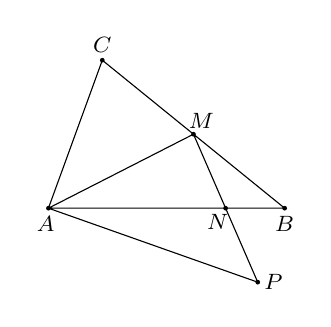
\begin{tikzpicture}[scale=1,>=stealth, font=\footnotesize, line join=round, line cap=round,declare function={h=2;}]
				\path
				(0,0) coordinate (A)
				(3,0) coordinate (B)
				(A)+(70:h) coordinate (C)
				(barycentric cs:C=1,B=1)coordinate(M)
				(barycentric cs:A=1,B=3)coordinate(N)
				(barycentric cs:A=0.5,B=1,C=-0.5)coordinate(P)
				;
				\draw (A)--(B)--(C)--(A)--(M)--(P)--cycle;
				\foreach \p/\g in{A/-100,B/-90,C/90,M/60,N/-120,P/0}
				\fill(\p)circle(.03)node[shift={(\g:.2)},scale=1]{$\p$};
			\end{tikzpicture}
		\end{center}
		\begin{itemchoice}
			\itemch \textbf{Đúng}.\\
			Vì $M$ là trung điểm của cạnh $BC$ nên
			\begin{align*}
				\overrightarrow{MB}+\overrightarrow{MC}=\overrightarrow{0} \Leftrightarrow \overrightarrow{AB}-\overrightarrow{AM}+\overrightarrow{AC}-\overrightarrow{AM}=\overrightarrow{0} \Leftrightarrow \overrightarrow{AM}=\dfrac{1}{2}\overrightarrow{AB}+\dfrac{1}{2}\overrightarrow{AC}.\tag{1}
			\end{align*}
			\itemch \textbf{Đúng}.\\
			Vì $N$ là điểm trên cạnh $AB$ sao cho $AN=3NB$ nên
			\begin{align*}
				\overrightarrow{AN}=3\overrightarrow{NB} \Leftrightarrow \overrightarrow{AN}=3\left(\overrightarrow{AB}-\overrightarrow{AN}\right) \Leftrightarrow \overrightarrow{AN}=\dfrac{3}{4}\overrightarrow{AB}. \tag{2}
			\end{align*}
			\itemch \textbf{Sai}.\\
			Từ $(1)$ và $(2)$, ta được
			\begin{align*}
				\overrightarrow{AN}-\overrightarrow{AM}=\dfrac{1}{4}\overrightarrow{AB}-\dfrac{1}{2}\overrightarrow{AC} \Leftrightarrow \overrightarrow{MN}=\dfrac{1}{4}\overrightarrow{AB}-\dfrac{1}{2}\overrightarrow{AC}. \tag{3}
			\end{align*}
			\itemch \textbf{Đúng}.\\
			Ta có
			\allowdisplaybreaks
			\begin{eqnarray*}
				&&\overrightarrow{AP}=\overrightarrow{AB}-\dfrac{1}{2}\overrightarrow{AC}\\
				&\Leftrightarrow& \overrightarrow{AM}+\overrightarrow{MP}=\overrightarrow{AB}-\dfrac{1}{2}\overrightarrow{AC}\\
				&\Leftrightarrow& \dfrac{1}{2}\overrightarrow{AB}+\dfrac{1}{2}\overrightarrow{AC}+\overrightarrow{MP}=\overrightarrow{AB}-\dfrac{1}{2}\overrightarrow{AC}\quad (\text{do }(1))\\
				&\Leftrightarrow& \overrightarrow{MP}=\dfrac{1}{2}\overrightarrow{AB}-\overrightarrow{AC}\\
				&\Leftrightarrow& \overrightarrow{MP}=2\overrightarrow{MN} \quad (\text{do }(3)).
			\end{eqnarray*}
			Từ đó suy ra ba điểm $M$, $N$, $P$ thẳng hàng.
		\end{itemchoice}
	}
\end{ex}
%==========Câu 3
\begin{ex}%[0-HK1-KN-5-SocSon-HaNoi-2324]%[VN-MT-6,VM024]%[0D1V3-3]
	Cho $A=\left\{x\in\mathbb{R}\ \Big|\ |x-m|\le 25\right\}$; $B=\left\{x\in\mathbb{R}\ \Big|\ | x|\ge 2\,020\right\}$.
	\choiceTF
	{\True $B=(-\infty;-2\, 020]\cup[2\,020;+\infty)$}
	{\True $\mathrm{C}_{\mathbb{R}} B=(-2\, 020;2\, 020)$}
	{Với mỗi $m\in\mathbb{N}$, tập hợp $A$ có $51$ phần tử}
	{\True Có $3\,989$ giá trị nguyên $m$ thỏa mãn $A\cap B=\varnothing$}
	\loigiai{
		\begin{itemchoice}
			\itemch \textbf{Đúng}.\\
			Ta có
			\allowdisplaybreaks
			\begin{eqnarray*}
				B&=&\left\{x\in\mathbb{R}\ \Big|\ |x|\ge 2\,020\right\}\\
				&=&\left\{x\in\mathbb{R}\ \Big|\ x\le -2\,020\text{ hoặc }x\ge2\,020\right\}\\
				&=&(-\infty;-2\,020]\cup[2\,020;+\infty).
			\end{eqnarray*}
			\itemch \textbf{Đúng}.\\
			Ta có $\mathrm{C}_{\mathbb{R}} B=\mathbb{R}\setminus\big((-\infty;-2\,020]\cup[2\,020;+\infty)\big)=(-2\, 020;2\, 020)$.
			\itemch \textbf{Sai}.\\
			Ta có\\ $A=\left\{x\in\mathbb{R}\ \Big|\ |x-m|\le 25\right\}=\left\{x\in\mathbb{R}\ \Big|\ m-25\le x\le m+25\right\}=\left[m-25;m+25\right]$.\\
			Do đó, tập hợp $A$ có vô số phần tử, với mọi $m\in\mathbb{N}$.
			\itemch \textbf{Đúng}.\\
			$A\cap B=\varnothing$ khi và chỉ khi $-2020<m-25<m+25<2020 \Leftrightarrow -1995<m<1995$.\\
			Do $m$ nguyên nên $m\in\left\{-1994;-1993;-1992;\ldots;1994\right\}$.\\
			Vậy có $3\,989$ giá trị nguyên $m$ thỏa mãn $A\cap B=\varnothing$.
		\end{itemchoice}
	}
\end{ex}
%==========Câu 4
\begin{ex}%[0-HK1-KN-5-SocSon-HaNoi-2324]%[VN-MT-6,VM024]%[0H9C2-5]
	Trong mặt phẳng với hệ tọa độ $Oxy$, cho tam giác $ABC$ với $A(-1;2)$, $B(2;6)$, $C(3;4)$.
	\choiceTF
	{\True Tam giác $ABC$ vuông tại $C$}
	{Diện tích tam giác $ABC$ bằng $10$}
	{Gọi $H$ là điểm thuộc đường thẳng $BC$ sao cho $AH$ ngắn nhất. Khi đó, $H\left(\dfrac{5}{2};5\right)$}
	{Tâm của đường tròn ngoại tiếp tam giác $OAB$ là $I\left(\dfrac{1}{3};\dfrac{8}{3}\right)$}
	\loigiai{
		\begin{itemchoice}
			\itemch \textbf{Đúng}.\\
			Ta có $\overrightarrow{CA}=(-4;-2)$, $\overrightarrow{CB}=(-1;2)$. Do đó,
			\begin{align*}
				\overrightarrow{CA}\cdot \overrightarrow{CB}=(-4)\cdot (-1)+(-2)\cdot 2=0 \Rightarrow \overrightarrow{CA}\perp\overrightarrow{CB}.
			\end{align*}
			Vậy $\triangle ABC$ vuông tại $C$.
			\itemch \textbf{Sai}.\\
			Ta có $CA=\sqrt{(-4)^2+(-2)^2}=\sqrt{20}=2\sqrt{5}$; $CB=\sqrt{(-1)^2+2^2}=\sqrt{5}$.\\
			Vậy $S_{\triangle ABC}=\dfrac{1}{2}CA\cdot CB=\dfrac{1}{2}\cdot 2\sqrt{5}\cdot \sqrt{5}=5$.
			\itemch \textbf{Sai}.\\
			Ta có $H\in BC$, $AC\perp BC$ $\Rightarrow$ $AH\ge AC$.\\
			Đẳng thức xảy ra khi và chỉ khi $H\equiv C$.\\
			Vậy $H(3;4)$.
			\itemch \textbf{Sai}.\\
			$I(x;y)$ là tâm của đường tròn ngoại tiếp tam giác $OAB$ khi và chỉ khi
			\allowdisplaybreaks
			\begin{eqnarray*}
				&& \heva{&IO=IA\\ &IO=IB}\\
				&\Leftrightarrow& \heva{&OI^2=AI^2\\ &OI^2=BI^2}\\
				&\Leftrightarrow& \heva{&x^2+y^2=(x+1)^2+(y-2)^2\\ &x^2+y^2=(x-2)^2+(y-6)^2}\\
				&\Leftrightarrow& \heva{&-2x+4y=5\\ &4x+12y=40}\\
				&\Leftrightarrow& \heva{&x=\dfrac{5}{2}\\ &y=\dfrac{5}{2}.}
			\end{eqnarray*}
			Vậy $I\left(\dfrac{5}{2};\dfrac{5}{2}\right)$.
		\end{itemchoice}
	}
\end{ex}

\Closesolutionfile{ans}
%================================PHẦN III
\caukq
\Opensolutionfile{ans}[ans/0-HK1-KN-5-SocSon-HaNoi-2324-Phan-III]
\setcounter{ex}{0}
%==========Câu 1
\begin{ex}%[0-HK1-KN-5-SocSon-HaNoi-2324]%[VN-MT-6,VM024]%[0D6N3-5]
	Điểm thi học kì môn Toán của một nhóm bạn như sau
	\begin{center}
		\begin{tabular}{|c|c|c|c|c|c|c|c|}
			\hline
			$8$ & $9$ & $7$ & $10$ & $7$ & $5$ & $7$ & $8$ \\ \hline
		\end{tabular}
	\end{center}
	Tìm mốt của mẫu số liệu trên.
	\shortans{$7$}
	\loigiai{
		Ta có bảng phân bố tần số như sau
		\begin{center}
			\begin{tabular}{|l|c|c|c|c|c|}
				\hline
				Điểm & $5$ & $7$ & $8$ & $9$ & $10$ \\ \hline
				Tần số & $1$ & $3$ & $2$ & $1$ & $1$\\ \hline
			\end{tabular}
		\end{center}
		Vậy mốt của mẫu số liệu trên là $7$.
	}
\end{ex}
%==========Câu 2
\begin{ex}%[0-HK1-KN-5-SocSon-HaNoi-2324]%[VN-MT-6,VM024]%[0H4N2-1]
	Cho tam giác $ABC$ có $AB=10$ và $\widehat{C}=30^\circ$. Tính bán kính $R$ của đường tròn ngoại tiếp $\triangle ABC$.
	\shortans{$10$}
	\loigiai{
		Theo định lý sin trong tam giác, ta có $\dfrac{AB}{\sin C}=2R$. Suy ra $R=\dfrac{AB}{2\sin C}=10$.
	}
\end{ex}
%==========Câu 3
\begin{ex}%[0-HK1-KN-5-SocSon-HaNoi-2324]%[VN-MT-6,VM024]%[0H9H1-5]
	Cho $\overrightarrow{a}=(x;2)$, $\overrightarrow{b}=(-5;1)$, $\overrightarrow{c}=(x;7)$. Tìm $x$ biết $\overrightarrow{c}=2\overrightarrow{a}+3\overrightarrow{b}$.
	\shortans{$15$}
	\loigiai{
		Vì $\overrightarrow{c}=2\overrightarrow{a}+3\overrightarrow{b}$ nên ta có $\heva{&x=2\cdot x+3\cdot (-5)\\ &7=2\cdot 2+3\cdot 1}$ $\Leftrightarrow$ $x=15$.
	}
\end{ex}
%==========Câu 4
\begin{ex}%[0-HK1-KN-5-SocSon-HaNoi-2324]%[VN-MT-6,VM024]%[0H5V3-6]
	Cho hình vuông $ABCD$ có cạnh bằng $2$. Tính độ dài của vectơ tổng $2\overrightarrow{DA}+\dfrac{1}{2}\overrightarrow{DC}$ (kết quả làm tròn đến chữ số thập phân thứ hai).
	\shortans{$4{,}12$}
	\loigiai{
		\begin{center}
			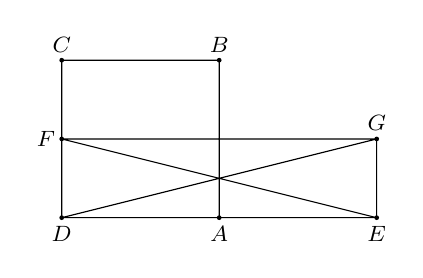
\begin{tikzpicture}[scale=1,>=stealth, font=\footnotesize, line join=round, line cap=round,declare function={h=2;}]
				\path
				(0,0) coordinate (D)
				(2,0) coordinate (A)
				(2,2) coordinate (B)
				(barycentric cs:A=-1,D=1,B=1)coordinate(C)
				(barycentric cs:A=2,D=-1)coordinate(E)
				(barycentric cs:D=1,C=1)coordinate(F)
				(barycentric cs:D=-1,E=1,F=1)coordinate(G)
				;
				\draw (D)--(A)--(B)--(C)--(D)--(G)--(F)--(E)--(G) (A)--(E);
				\foreach \p/\g in{A/-90,B/90,C/90,D/-90,E/-90,F/180,G/90}
				\fill(\p)circle(.03)node[shift={(\g:.2)},scale=1]{$\p$};
			\end{tikzpicture}
		\end{center}\vspace{-0.3cm}
		Gọi $E$ là điểm sao cho $\overrightarrow{DE}=2\overrightarrow{DA}$. Suy ra $DE=2DA=4$.\\
		Gọi $F$ là điểm sao cho $\overrightarrow{DF}=\dfrac{1}{2}\overrightarrow{DA}$. Suy ra $DE=\dfrac{1}{2}DC=1$.\\
		Gọi $G$ là đỉnh thứ tư của hình chữ nhật $EDFG$.\\
		Khi đó,
		\begin{align*}
			\left|2\overrightarrow{DA}+\dfrac{1}{2}\overrightarrow{DC}\right|=\left|\overrightarrow{DE}+\overrightarrow{DF}\right|=\left|\overrightarrow{DG}\right|=DG=\sqrt{DE^2+EG^2}=\sqrt{DE^2+DF^2}=\sqrt{17}\approx 4{,}12.
		\end{align*}
	}
\end{ex}
%==========Câu 5
\begin{ex}%[0-HK1-KN-5-SocSon-HaNoi-2324]%[VN-MT-6,VM024]%[0H9V2-5]
	Trong mặt phẳng với hệ tọa độ $Oxy$, cho hai điểm $A(2;4)$, $B(1;1)$. Biết $M(a;b)$ là điểm thỏa mãn tam giác $ABM$ vuông cân tại $B$. Tính giá trị $T=3a+4b$.
	\shortans{$2$}
	\loigiai{
		Ta có $\overrightarrow{BA}=(1;3)$, $\overrightarrow{BM}=(a-1;b-1)$.\\
		Tam giác $ABM$ vuông cân tại $B$ khi và chỉ khi
		\allowdisplaybreaks
		\begin{eqnarray*}
			&&\heva{&\overrightarrow{BA}\cdot \overrightarrow{BM}=0\\ &BM=BA} \\
			&\Leftrightarrow& \heva{&\overrightarrow{BA}\cdot \overrightarrow{BM}=0\\ &BM^2=BA^2} \\
			&\Leftrightarrow& \heva{&a-1+3(b-1)=0\\ &(a-1)^2+(b-1)^2=10} \\
			&\Leftrightarrow& \heva{&a-1=-3(b-1)\\ & 10(b-1)^2=10} \\
			&\Leftrightarrow& \heva{&(b-1)^2=1\\ &a=-3b+4} \\
			&\Leftrightarrow& \hoac{&\heva{&b=2\\ &a=-2}\\ &\heva{&b=0\\ &a=4.}}
		\end{eqnarray*}
		Vì $a<0$ nên $a=-2$ và $b=2$.\\
		Vậy $T=3a+4b=3\cdot (-2)+4\cdot 2=2$.
	}
\end{ex}
%==========Câu 6
\begin{ex}%[0-HK1-KN-5-SocSon-HaNoi-2324]%[VN-MT-6,VM024]%[0D6H4-2]
	Nhiệt độ của một thành phố trong $10$ ngày qua được ghi lại lần lượt là
	\begin{center}
		\begin{tabular}{|c|c|c|c|c|c|c|c|c|c|}
			\hline
			$24$ & $21$ & $30$ & $34$ & $28$ & $35$ & $33$ & $36$ & $25$ & $27$ \\ \hline
		\end{tabular}
	\end{center}
	Hãy tính khoảng tứ phân vị của mẫu số liệu.
	\shortans{$9$}
	\loigiai{
		Ta sắp xếp mẫu số liệu theo thứ tự không giảm như sau
		\begin{center}
			\begin{tabular}{|c|c|c|c|c|c|c|c|c|c|}
				\hline
				$21$ & $24$ & $25$ & $27$ & $28$ & $30$ & $33$ & $34$ & $35$ & $36$ \\ \hline
			\end{tabular}
		\end{center}
		Mẫu số liệu gồm $10$ giá trị nên số trung vị là $Q_2=\dfrac{(28+30)}{2}=29$.\\
		Nửa số liệu bên trái là $21$; $24$; $25$; $27$; $28$ gồm $5$ giá trị, số chính giữa là $25$ nên $Q_1=25$.\\
		Nửa số liệu bên phải là $30$; $33$; $34$; $35$; $36$ gồm $5$ giá trị, số chính giữa là $34$ nên $Q_3=34$.\\
		Khoảng tứ phân vị của mẫu số liệu bằng $\Delta_Q=Q_3-Q_1=34-25=9$.
	}
\end{ex}
\Closesolutionfile{ans}
% \begin{indapan}
% 	{ans/0-HK1-KN-5-SocSon-HaNoi-2324}
% \end{indapan}